\RequirePackage{ifpdf}
\documentclass[a4paper,11pt]{scrartcl} 
\usepackage[margin=2.5cm]{geometry}
\usepackage{multirow}
\usepackage{tabularx} 
\usepackage{rotating,graphicx} 
\usepackage{appendix} 
\usepackage{makecell}
\usepackage{amsmath}
\usepackage{amssymb}
\usepackage{cite}
%\ifpdf
%  \usepackage[pdftex]{graphicx}
%\else
%  \usepackage[dvips]{graphicx}
%\fi
%\usepackage[utf8]{inputenc}
\usepackage[T1]{fontenc}
\usepackage{amsmath}
\usepackage[amssymb]{SIunits}
\usepackage{hyperref}

\usepackage{lineno}
\linenumbers

\usepackage{xcolor}

% $Id: commands.tex 909 2013-06-03 14:10:59Z rpreghen $
% Adaptation of a file originally by Roberto Preghenella (thanks!) 
%==========================================================%
\newcommand{\btwo}{\ensuremath{B_{2}}}
\newcommand{\bthree}{\ensuremath{B_{3}}}
\newcommand{\bA}{\ensuremath{B_{A}}}
\newcommand{\bthreeLambda}{$B_{3, \Lambda}$}

%nuclei and hypernuclei
\newcommand{\tritium}{\ensuremath{{}^{3}\mathrm{H}}}
\newcommand{\hethree}{\ensuremath{{}^{3}\mathrm{He}}}
\newcommand{\hefour}{\ensuremath{{}^{4}\mathrm{He}}}
\newcommand{\hthreelambda}{\ensuremath{{}^{3}_{\Lambda}\mathrm{H}}}
\newcommand{\hfourlambda}{\ensuremath{{}^{4}_{\Lambda}\mathrm{H}}}
\newcommand{\hfourtwolambda}{\ensuremath{{}^{4}_{\Lambda\Lambda}\mathrm{H}}}
\newcommand{\hefourlambda}{\ensuremath{{}^{4}_{\Lambda}\mathrm{He}}}

\newcommand{\antitritium}{\ensuremath{{}^{3}\overline{\mathrm{He}}}}
\newcommand{\antihethree}{\ensuremath{{}^{3}\overline{\mathrm{He}}}}
\newcommand{\antihefour}{\ensuremath{${}^{4}$\overline{\mathrm{He}}}}
\newcommand{\antihthreelambda}{\ensuremath{{}^{3}_{\Lambda}\overline{\mathrm{He}}}}
\newcommand{\antihfourlambda}{\ensuremath{{}^{4}_{\Lambda}\overline{\mathrm{H}}}}
\newcommand{\antihefourlambda}{\ensuremath{{}^{4}_{\Lambda}\overline{\mathrm{He}}}}
\newcommand{\antihfourtwolambda}{\ensuremath{{}^{4}_{\Lambda\Lambda}\overline{\mathrm{H}}}}

\newcommand{\dradius}{\ensuremath{r_{d}}}
\newcommand{\rperp}{\ensuremath{R_{\perp}}}
\newcommand{\rpar}{\ensuremath{R_{\|}}}



%==========================================================%
\newcommand{\Om}{$\Omega^-$}
\newcommand{\Mo}{$\overline{\Omega}^+$}
\newcommand{\X}{$\Xi^-$}
\newcommand{\Ix}{$\overline{\Xi}^+$}
\newcommand{\Xis}{$\Xi^{\pm}$}
\newcommand{\Oms}{$\Omega^{\pm}$}
\newcommand{\meanpt}{$\langle p_\mathrm{t}\rangle$}
\newcommand{\nineH}{$\sqrt{s}~=~0.9$~TeV}
\newcommand{\seven}{$\sqrt{s}~=~7$~TeV}
\newcommand{\twoH}{$\sqrt{s}~=~0.2$~TeV}
\newcommand{\dndy}{d$N$/d$y$}
\newcommand{\LT}{L{\'e}vy-Tsallis}
\newcommand{\GeVc}{GeV/$c$}
\newcommand{\MeVc}{MeV/$c$}
\newcommand{\GeVcs}{GeV/$c$ }
\newcommand{\MeVcs}{MeV/$c$ }
\newcommand{\GeVmass}{GeV/$c^2$}
\newcommand{\MeVmass}{MeV/$c^2$}
\newcommand{\allpart}{\kzero, \lmb, \almb, \X, \Ix, \Om and \Mo}

\newcommand{\ITS}          {\rm{ITS }}
\newcommand{\TOF}          {\rm{TOF }}
\newcommand{\ZDC}          {\rm{ZDC }}
\newcommand{\ZDCs}         {\rm{ZDCs }}
\newcommand{\ZNA}          {\rm{ZNA }}
\newcommand{\ZNC}          {\rm{ZNC }}
\newcommand{\SPD}          {\rm{SPD }}
\newcommand{\SDD}          {\rm{SDD }}
\newcommand{\SSD}          {\rm{SSD }}
\newcommand{\TPC}          {\rm{TPC }}
\newcommand{\VZERO}        {\rm{VZERO }}
\newcommand{\VZEROA}       {\rm{VZERO-A }}
\newcommand{\VZEROC}       {\rm{VZERO-C }}
\newcommand{\pip}          {\ensuremath{\pi^{+}}}
\newcommand{\pim}          {\ensuremath{\pi^{-}}}
\newcommand{\pipm}          {\ensuremath{\pi^{\pm}}}
\newcommand{\kap}          {\ensuremath{\mathrm{K}^{+}}}
\newcommand{\kam}          {\ensuremath{\mathrm{K}^{-}}}
\newcommand{\kapm}          {\ensuremath{\mathrm{K}^{\pm}}}
\newcommand{\p}               {$\rm p$}
\newcommand{\pbar}         {$\rm\overline{p}$}
\newcommand{\kzero}        {\ensuremath{{\rm K}^{0}_{S}}}
\newcommand{\kstar}        {\ensuremath{{\rm K}^{*0}}}
\newcommand{\lmb}          {\ensuremath{\Lambda}}
\newcommand{\almb}         {\ensuremath{\overline{\Lambda}}}
%this is another analysis...
%\newcommand{\allpart}      {$\pi^{\pm}$, K$^{\pm}$, \kzero, p(\pbar) and \lmb(\almb)}
%\newcommand{\degree}       {$^{\rm o}$}
\newcommand{\dg}           {\mbox{$^\circ$}}
\newcommand{\dedx}         {\ensuremath{\mathrm{d}E/\mathrm{d}x}}
\newcommand{\pp}           {pp}
\newcommand{\ppbar}        {\mbox{$\mathrm {p\overline{p}}$}}
\newcommand{\PbPb}         {\mbox{Pb--Pb}}
\newcommand{\pPb}          {\mbox{p--Pb}}
\newcommand{\AuAu}         {\mbox{Au--Au}}
\newcommand{\pseudorap}    {\mbox{$\left | \eta \right | $}}
\newcommand{\dNdeta}       {\ensuremath{\mathrm{d}N_\mathrm{ch}/\mathrm{d}\eta}}

\newcommand{\avdNdeta}       {\ensuremath{\left<\mathrm{d}N_\mathrm{ch}/\mathrm{d}\eta\right>}}
\newcommand{\dNchdy}         {\ensuremath{\mathrm{d}N_\mathrm{ch}/\mathrm{d}y}}
\newcommand{\dNdy}         {\ensuremath{\mathrm{d}N/\mathrm{d}y} }
\newcommand{\dNdyst}       {\ensuremath{\sqrt{\frac{dN_\pi/dy}{s_T}}}}
\newcommand{\dNdetatr}     {\mathrm{d}N_\mathrm{tracklets}/\mathrm{d}\eta}
\newcommand{\dNdetar}[1]   {\mathrm{d}N_\mathrm{ch}/\mathrm{d}\eta\left.\right|_{|\eta|<#1}}
\newcommand{\lum}          {\, \mbox{${\rm cm}^{-2} {\rm s}^{-1}$}}
%\newcommand{\barn}         {\, \mbox{${\rm barn}$}}
\newcommand{\m}            {\, \mbox{${\rm m}$}}
\newcommand{\ncls}         {\ensuremath{N_{cls}}}
\newcommand{\nsigma}       {\ensuremath{n\sigma}}
\newcommand{\dcaxy}        {\ensuremath{{\rm DCA}_{xy}} }
\newcommand{\dcaz}         {\ensuremath{{\rm DCA}_{z}} }
\newcommand{\EcrossB}      {E$\times$B}%{\ensuremath{{\rm E}\times{\rm B}}}
\newcommand{\bb}           {Bethe-Bloch}
\newcommand{\s}            {\ensuremath{\sqrt{s}}}
\newcommand{\pt}           {\ensuremath{p_{\mathrm{T}}}}
\newcommand{\pts}           {\ensuremath{p_{\rm T}} }
\newcommand{\hlab}         {\ensuremath{\eta_{\rm lab}}}
\newcommand{\ynn}         {\ensuremath{y_{\rm NN}}}
\newcommand{\ycms}         {\ensuremath{y_{\rm CMS}}}
\newcommand{\ylab}         {\ensuremath{y_{\rm lab}}}
\newcommand{\ppi}          {\ensuremath{{\rm p}/\pi}}
\newcommand{\kpi}          {\ensuremath{{\rm K}/\pi}}
\newcommand{\lpi}          {\ensuremath{{\rm \Lambda}/\pi}}
%\newcommand{\ppi}          {\ensuremath{(\pi^+ + \pi^-)/({\rm K}^+ + {\rm K}^-)}}
%\newcommand{\kpi}          {\ensuremath{({\rm p} + {\rm \bar p})/({\rm K}^+ + {\rm K}^-)}}
\newcommand{\mt}           {\ensuremath{m_{\rm T}}}
\newcommand{\snn}          {\ensuremath{\sqrt{s_{\rm NN}}}}
\newcommand{\snnbf}        {\ensuremath{\mathbf{{\sqrt{s_{\mathbf NN}}}}}}
\newcommand{\sonly}        {\ensuremath{\sqrt{s}}}
\newcommand{\Npart}        {\ensuremath{N_\mathrm{part}}}
\newcommand{\avNpart}      {\ensuremath{\langle N_\mathrm{part} \rangle}}
\newcommand{\avNpartdata}  {\ensuremath{\langle N_\mathrm{part}^{\rm data} \rangle}}
\newcommand{\Ncoll}        {\ensuremath{N_\mathrm{coll}}}
\newcommand{\Dnpart}       {\ensuremath{D\left(\Npart\right)}}
\newcommand{\DnpartExp}    {\ensuremath{D_{\rm exp}\left(\Npart\right)}}
\newcommand{\dNdetapt}     {\ensuremath{\dNdeta\,/\left(0.5\Npart\right)}}
\newcommand{\dNdetaptr}[1] {\ensuremath{\dNdetar{#1}\,/\left(0.5\Npart\right)}}
\newcommand{\dNdetape}     {\left(\ensuremath{\dNdeta\right)/\left(\avNpart/2\right)}}
\newcommand{\dNdetaper}[1] {\ensuremath{\dNdetar{#1}\,/\left(\avNpart/2\right)}}
\newcommand{\dndydpt}      {\ensuremath{{\rm d}^2N/({\rm d}y {\rm d}p_{\rm t})}}
\newcommand{\abs}[1]       {\ensuremath{\left|#1\right|}}
\newcommand{\signn}        {\ensuremath{\sigma^{\rm inel.}_{\rm NN}}}
\newcommand{\vz}           {\ensuremath{V_{z}}}
\newcommand{\Tfo}          {\ensuremath{{T}_{\rm kin}}}
\newcommand{\Tch}          {\ensuremath{{T}_{\rm ch}}}
\newcommand{\bT}           {\ensuremath{\beta_{\rm T}}}
\newcommand{\avbT}         {\ensuremath{\left< \beta_{\rm T}\right>}}
\newcommand{\avpT}         {\ensuremath{\left< \pt \right>}\xspace}
\newcommand{\muB}          {\ensuremath{\mu_{B}}}
\newcommand{\stat}         {({\it stat.})}
\newcommand{\syst}         {({\it sys.})}
\newcommand{\Fig}[1]       {Fig.~\ref{#1}}
\newcommand{\Figure}[1]    {Figure~\ref{#1}}
\newcommand{\Ref}[1]       {Ref.~\cite{#1}}
\newcommand{\green}[1]     {\textcolor{green}{#1}}
\newcommand{\blue}[1]      {\textcolor{blue}{#1}}
\newcommand{\red}[1]       {\textcolor{red}{#1}}
\newcommand{\white}[1]     {\textcolor{white}{#1}}
\newcommand{\gevc}         {\ensuremath{{\rm GeV}/c}}
\newcommand{\mevc}         {\ensuremath{{\rm MeV}/c}}
\newcommand{\gevcs}         {\ensuremath{{\rm GeV}/c} }
\newcommand{\mevcs}         {\ensuremath{{\rm MeV}/c} }
\newcommand{\avg}[1]       {\ensuremath{\left\langle#1\right\rangle}}

\newcommand {\dEdx}      {d\textit{E}/d\textit{x}\xspace}
\newcommand {\Zvtx}   {\ensuremath{Z_\mathrm{vtx}}\xspace}
\newcommand {\pT}   {\pt}

\newcommand {\proton}     		{\ensuremath{p}}
\newcommand {\electron}   		{\Pe}
\newcommand {\pion}    	  		{\ensuremath{\pi}}
\newcommand {\kaon}       		{\ensuremath{K}}
\newcommand {\KTopi}      		{\kaon/\pion}
\newcommand {\pTopi}      		{\proton/\pion}
\newcommand {\KzeroShort} 		{\PKzS}
\newcommand {\lambdaBaryon} 	{\PGL}
\newcommand {\antiLambdaBaryon} {\PAGL}
\newcommand {\gammaPhoton} 		{\PGg}
\newcommand {\Nevt}      {\ensuremath{N_\mathrm{evt}}\xspace}
\newcommand {\NevtMB}  {\ensuremath{N_\mathrm{evt|MB}}\xspace}
\newcommand {\NevtMBVTX}  {\ensuremath{N_\mathrm{evt|(MB\, \&\, Vtx)}}\xspace}
\newcommand {\NevtMBVTXZ}  {\ensuremath{N_\mathrm{evt|(MB\, \& Vtx\, \&\, \textit{Z}_{vtx})}}\xspace}
\newcommand {\NevtINEL}  {\ensuremath{N_\mathrm{evt}(\textsc{inel})}\xspace}
\newcommand {\fPrim}       {\ensuremath{f_{\mathrm{prim}}}\xspace}
\newcommand {\NPrim}     {\ensuremath{N_{\mathrm{prim}}}\xspace}
\newcommand {\NSec}      {\ensuremath{N_{\mathrm{sec}}}\xspace}
\newcommand {\NPrimTilde}     {\ensuremath{\widetilde{N}_{\mathrm{prim}}}\xspace}
\newcommand {\NSecTilde}      {\ensuremath{\widetilde{N}_{\mathrm{sec}}}\xspace}
\newcommand {\NTilde}      {\ensuremath{\widetilde{N}}\xspace}

\newcommand{\pPiplus}{\ensuremath{{\pi}^{+}}\xspace}
\newcommand{\pPiminus}{\ensuremath{{\pi}^{-}}\xspace}
\newcommand{\sPi}{\ensuremath{{\pi}}\xspace}
\newcommand{\pKplus}{\ensuremath{{\rm K}^{+}}\xspace}
\newcommand{\pKminus}{\ensuremath{{\rm K}^{-}}\xspace}
\newcommand{\sProton}{\ensuremath{\rm p}\xspace}
\newcommand{\pProton}{\ensuremath{\rm p}\xspace}
\newcommand{\apProton}{\ensuremath{\overline{\rm p}}\xspace}
\newcommand{\sPr}{\ensuremath{\rm p}\xspace}
\newcommand{\sKzero}{\ensuremath{2{\rm K}^{0}_{S}}\xspace}
\newcommand{\pKzero}{\ensuremath{{\rm K}^{0}_{S}}\xspace}
\newcommand{\sLambda}{\ensuremath{\Lambda}\xspace}
\newcommand{\pLambda}{\ensuremath{\Lambda}\xspace}

\newcommand{\LtoKzero}{\ensuremath{\Lambda}/\ensuremath{{\rm K}^{0}_{S}}\xspace}
\newcommand{\apLambda}{\ensuremath{\overline{\Lambda}}\xspace}
\newcommand{\sXi}{\ensuremath{\Xi}\xspace}
\newcommand{\pXi}{\ensuremath{\Xi^{-}}\xspace}
\newcommand{\apXi}{\ensuremath{\overline{\Xi}^{+}}\xspace}
\newcommand{\sOmega}{\ensuremath{\Omega}\xspace}
\newcommand{\pOmega}{\ensuremath{\Omega^{-}}\xspace}
\newcommand{\apOmega}{\ensuremath{\overline{\Omega}^{+}}\xspace}

\newcommand{\betaT}{\ensuremath{\langle \beta_{T}\rangle}\xspace}
\newcommand{\Tkin}{\ensuremath{T_{kin}}\xspace}

\renewcommand{\labelitemi} {$-$}
%==========================================================%
%%% inline warnings for internal discussion 
%\newcommand{\warn}[1]      {\textbf{\textcolor{red}{[#1]}}}
\newcommand{\warn}[1]      {{\small\textbf{\textcolor{red}{(!\footnote{\textbf{(!)}~#1})}}}}
%\newcommand{\warn}[1]      {{\small\textbf{(!\footnote{\textbf{(!)}~#1})}}\marginpar{\textbf{---}}}
\newcommand{\todo}[1]      {\textbf{\textcolor{red}{[TODO: #1]}}}
%%% fake numbers
\newcommand{\fake}[1]      {\textbf{\textcolor{red}{#1}}}
%\newcommand{\fake}[1]      {#1}
\newcommand{\final}[1]     {\textbf{\textcolor{blue}{#1}}}
\newcommand{\prelim}[1]    {\textbf{\textcolor{magenta}{#1}}}
\renewcommand{\mod}[1]       {\textbf{\textcolor{red}{#1}}}


\begin{document}
\begin{center}

{\Large \textbf{Testing coalescence and statistical-thermal production scenarios for (anti-)(hyper-)nuclei and exotic QCD objects at LHC energies}}

\medskip

F. Bellini$^{1}$ and A. Kalweit$^{1}$
\\$^{1}$CERN, Switzerland
\medskip

15th July 2018
\end{center}

\bigskip

\begin{abstract}
(Anti-)(hyper-)nuclei are unique probes of the medium created in proton-proton, proton-Pb, and Pb--Pb collisions at the energies available at the Large Hadron Collider (LHC). Their production is typically discussed within the framework of coalescence and thermal-statistical production models. While it is often argued that these two approaches are not distinguishable, we present a detailed study of both theories which reveals large differences between the two scenarios for the production of objects with extended wave-functions. Both models give similar predictions and show similar agreement with experimental data for (anti-)deuterons and (anti-)\hethree\ nuclei, but they largely differ in their description of (anti-)hyper-triton production.
The thermal-statistical model is found to be in agreement with results in central Pb--Pb collisions even though fragile objects such as light (anti-)(hyper-)nuclei should be destroyed in hadronic interactions after the chemical freeze-out of the system. Our findings highlight the unique potential of ultra-relativistic heavy-ion collisions as a laboratory to clarify the internal structure of exotic QCD objects and can serve as a basis for more refined calculations in the future.
\end{abstract}

\newpage

\section{Introduction} 
The formation of light anti- and hyper-nuclei in high energy proton-proton (pp), proton-nucleus (pA) and nucleus-nucleus (AA) collisions provides unique observables for the study of the system created in these collisions. In addition, these studies might shed light on the internal structure of the formed objects themselves. 
In this context, nuclei and hyper-nuclei are special objects with respect to non-composite hadrons (such as pions, protons, kaons, etc.), because their size (i.e. the extension of their wave-function) is comparable to a fraction or the whole system created in the collision~\cite{Adam:2015vna}.  
The relevant known properties of the objects under study here are summarised in Table \ref{tab:nucleusradii}.
As quantum-mechanical objects, their size is typically defined as the rms of their (charge) wave function, which corresponds to about 2 fm for light (anti-)nuclei as obtained from electron scattering experiments. Not much is known experimentally about the wave-functions of hyper-nuclei and other exotic QCD objects. For the hyper-triton, theoretical calculations indicate a rms of the wave-function of about 5 fm \cite{Nemura:1999qp}, which is significantly larger than that of non-strange $A = 3$ nuclei. This is driven by the average separation of the $\Lambda$ with respect to the two other nucleons which is expected to amount to up to 10 fm \cite{Nemura:1999qp}. Halo nuclei as $^{6}$He would therefore be an ideal complement to this study, but they remain out of the experimental reach in high-energy experiments in the near future.

Since about sixty years, coalescence models have been used to describe the formation of composite objects (see for instance \cite{Butler:1963, Kapusta:1980, Sato:1981ez, Nagle:1996vp, Scheibl:1998tk, Cho:2017dcy, Blum:2017qnn, Bazak:2018hgl, Zhao:2018lyf} and references therein).
Surprisingly, thermal-statistical models have been successful in describing not only light-flavour particle production, but also that of light (anti-)(hyper-)nuclei across a wide range of energies in nucleus-nucleus collisions \cite{Andronic:2017, Andronic:2010qu}. 
In this approach, particles are produced from a fireball in thermal and kinetic equilibrium with temperatures of the order of $T_{chem} \approx$ 156 MeV that are near the temperature of the QCD phase transition boundary, as predicted by lattice QCD calculations \cite{Bazavov:2014pvz,Bellwied:2013cta}. Particle abundances are fixed at chemical freeze-out, when inelastic collisions cease. Further elastic and pseudo-elastic collisions occur among the components of the expanding fireball, that can affect the spectral shapes and the measurable yields of short-lived (strongly decaying) hadronic resonances. Once the particle density of the system is so low that the mean free path for elastic collisions is larger than the size of the system, the fireball freezes-out kinetically. At LHC energies, this is seen to occur when the system has reached temperatures of the order of $T_{kin} \approx$ 90 MeV~\cite{Abelev:2013vea}. 
In such a dense and hot environment, composite objects with binding energies that are small with respect to the temperature of the system, appear as ``fragile'' objects. For instance, the binding energy of the deuteron is $B_{E, d}$ = 2.2 MeV $\ll T_{chem}, T_{kin}$.
As a matter of fact, the cross-section for pion-induced deuteron breakup is significantly larger than the typical (pseudo)-elastic cross-sections for the re-scattering of hadronic resonance decay products \cite{Garcilazo:1982yc, Bass:1998ca, Schukraft:2017nbn}. 
Similarly, the elastic cross-section which drives the deuteron spectra to kinetic equilibration in central heavy-ion collisions \cite{Acharya:2017dmc} is smaller than the breakup cross-section \cite{Garcilazo:1982yc, Bass:1998ca, Schukraft:2017nbn}.   
Based on this, the deuterons produced at chemical freeze-out would be expected not to survive the hadronic phase of the medium expansion, yet their production is measured to be consistent to the predictions from statistical-thermal models and they develop also a non-zero elliptic flow which is consistent with a common radial expansion together with the non-composite hadrons \cite{Acharya:2017dmc}. 
Several solutions have been proposed to solve this ``light (anti-)nuclei puzzle'': (a.) a sudden freeze-out at the QGP-hadron phase boundary, (b.) the thermal production of these objects as compact quark bags \cite{Andronic:2017}, and (c.) the coincidence of coalescence mechanism with that of thermal production \cite{Scheibl:1998tk, HeinzTorino}.
Data from rescattering of short-lived hadronic resonances indicate that the system undergoes a long-lasting hadronic phase before decoupling \cite{Abelev:2014uua}, thus strongly disfavouring hypothesis (a.). 
While hypothesis (b.) cannot presently be tested beyond the agreement of measured (anti-)nuclei production yields with statistical-thermal model predictions, hypothesis (c.) is scrutinised in the present work.

\begin{table}[htb]

\centering
\begin{tabularx}{\textwidth}{cccccccc}
\hline \hline \\[-2ex]
\makecell{Mass \\number } & Nucleus           &  \makecell{Compo-\\sition}               & $B_{E}$ (MeV)   & \makecell{Spin \\$J_{A}$} & \makecell{(Charge) \\rms radius \\ \rmsradius$^{meas}$~(fm)} &  \makecell{Harmonic \\ oscillator \\ size \\ parameter \\$r_{A}$ (fm) } & Refs. \\[1ex]  \hline \\[-2ex] 
      A = 2                     & d                                    & pn                                  &   2.224575 (9)     &     1   & 2.1413 $\pm$ 0.0025      &  3.2    &   \cite{VanDerLeun:1982bhg,Mohr:2015ccw}     \\[0.5ex]  \hline \\[-2ex]
\multirow{3}{*}{A = 3}  & \tritium 	                  & pnn                               &    8.4817986 (20) & 1/2   &  1.755  $\pm$ 0.086        &  2.15   &   \cite{Purcell:2015gtm}           \\
                                   & \hethree                         & ppn                                &   7.7180428  (23) & 1/2  & 1.959 $\pm$  0.030         &   2.48  &   \cite{Purcell:2015gtm} \\
                                   & \hthreelambda               & p$\Lambda$n                &    0.13 $\pm$ 0.05 & 1/2  &  4.9 --  10.0                    &  6.8 -- 14.1 & \cite{Davis:2005mb,Nemura:1999qp} \\[0.5ex]  \hline \\[-2ex]
\multirow{4}{*}{A = 4}  & \hefour                          & ppnn                              &    28.29566   (20)  &      0  &  1.6755 $\pm$ 0.0028  &  1.9  & \cite{1674-1137-41-3-030003,Angeli:2013epw} \\
                                   & \hfourlambda                & p$\Lambda$nn              &  2.04 $\pm$0.04   &   0   &    2.0 -- 3.8             & 2.4 -- 4.9  & \cite{Davis:2005mb,Nemura:1999qp} \\
                                   & \hfourtwolambda          &  p$\Lambda\Lambda$n &   0.39 -- 0.51         &    1     &    4.2 -- 7.1          & 5.5 -- 9.4  &   \cite{Nemura:1999qp} \\
                                   & \hefourlambda              & pp$\Lambda$n              &  2.39 $\pm$ 0.03  &    0   &    2.0 -- 3.8            & 2.4 -- 4.9  & \cite{Davis:2005mb,Nemura:1999qp}\\[0.5ex]  \hline \hline
\end{tabularx}
\caption{Properties of nuclei and hyper-nuclei with mass number $A \leq 4$. $B_{E}$ is the binding energy in MeV. The size of the nucleus is given in terms of the (charge) rms radius of the wavefunction, \rmsradius. The size parameter of the wave-function of the harmonic oscillator potential,  $r_{A}$, is chosen such that the measured/expected rms is approximately reproduced. Details are given in Appendix \ref{appendix:Sato}. Please note that the proton rms charge radius $\lambda_{p} = 0.879(8)$ fm \cite{bernauer10} is subtracted quadratically from the measured rms charge radius $\rmsradius^{meas}$ of the nucleus $\rmsradius = \sqrt{(\rmsradius^{meas})^2 - {\lambda_{p}^2}}$ to account for the finite extension of the constituents. Implicitly we assume here that $\lambda_{\Lambda}\approx \lambda_{n}\approx \lambda_{p}$.
 References are given in the last column. The spin of \hfourtwolambda\ is discussed in the text of~\cite{Nemura:1999qp}.}
\label{tab:nucleusradii}
\end{table}

To this purpose, we compare to models the existing data from the LHC. For the first time, these data allow for the systematic study of the light (anti-)(hyper-)nuclei production as a function of the system and object size. 
In the nucleon-coalescence approach, nuclei are formed at kinetic freeze-out by coalescence of nucleons that are nearby in space and have similar velocities. The coalescence model is reviewed in Section \ref{sec:coalescence}, starting from its simplest form (uncorrelated nucleon emission from a point-like source) to the full space-time evolution picture as discussed in \cite{Scheibl:1998tk}. In section \ref{sec:thermal}, a blast-wave parameterisation for particle transverse momentum spectra in combination with predictions from the statistical-thermal model for the yields is used as an alternative approach. 
The direct comparison of the two approaches and the comparison with data are discussed in section \ref{sec:comparison}.
We find that a systematic study of the coalescence parameter \bA~provides an important discrimination power between the two approaches. 
A comparison of the production rates of nuclei with similar mass but very different internal structure has already been suggested for the case of \hefour~and ${}^{4}\mathrm{Li}$ \cite{Bazak:2018hgl}. However, as the ${}^{4}\mathrm{Li}$ is not stable with respect to strong decay, its measurement is experimentally very challenging and probably less constraining than the comparison with hyper-nuclei proposed here.
We propose that \bA~is systematically measured in all collision systems by exploiting the large statistics sample that will be available with the LHC Run 3 \& 4, in order to rule out or support the aforementioned scenarios. As a matter of fact, the upcoming years of LHC data taking provide a unique opportunity for the final understanding of (anti-)(hyper-)nuclei production.
Setting a final word on the production mechanisms is not only in the interest of the heavy-ion community, but has a broader application in astrophysics and dark-matter searches, by representing an essential input for the measurement of (anti-)nuclei in space with ongoing \cite{Alcaraz:2000ss} and future \cite{AMS100, Aramaki:2015laa} experiments. 
In addition to this, the study of light(anti-)nuclei might serve as a baseline for understanding the debated nature of exotic states such as the X(3872), that has been interpreted as tetraquark state or hadronic molecule \cite{Esposito:2015fsa, Cho:2017dcy}.


\section{Coalescence approach} 
\label{sec:coalescence}

\subsection{Simple coalescence}
In the coalescence picture, nucleons produced in the collision coalesce into nuclei if they are close in space and have similar velocities \cite{Butler:1963,Kapusta:1980}. For a nucleus with mass number $A = Z + N$, the coalescence probability is typically quantified in terms of the coalescence parameter $B_{A}$, which is defined as

\begin{equation}
E_{A}\frac{\mathrm{d}^{3}N_{A}}{\mathrm{d}p_{A}^{3}}=B_{A}{\left(E_{\mathrm{p}}\frac{\mathrm{d}^{3}N_{\mathrm{p}}}{\mathrm{d}p_{\mathrm{p}}^{3}}\right)^{Z}\left\vert_{\vec{p}_{\mathrm{p}}=\frac{\vec{p}_{A}}{A}} \right.\;
   \left(E_{\mathrm{n}}\frac{\mathrm{d}^{3}N_{\mathrm{n}}}{\mathrm{d}p_{\mathrm{n}}^{3}}\right)^{N}}\left\vert_{\vec{p}_{\mathrm{n}}=\frac{\vec{p}_{A}}{A}} \right.\;
,    
\label{eq:BA}
\end{equation}

\noindent where $p_{\mathrm{p,n}}$ are the momenta of the proton and neutron and $E_{p,n}$ their energies.
Since in the LHC collision energy regime the number of produced protons and neutrons at midrapidity is expected to be equal, the equation simplifies to 
\begin{equation}
E_{A}\frac{\mathrm{d}^{3}N_{A}}{\mathrm{d}p_{A}^{3}}=B_{A}{\left(E_{\mathrm{p}}\frac{\mathrm{d}^{3}N_{\mathrm{p}}}{\mathrm{d}p_{\mathrm{p}}^{3}}\right)^{A}}\left\vert_{\vec{p}_{\mathrm{p}}=\frac{\vec{p}_{A}}{A}} \right..
\label{eq:BA}
\end{equation}
%
Moreover, the LHC is particularly suited for the production of anti-nuclei, since the number of baryons and anti-baryons is essentially equal at midrapidity \cite{Abbas:2013rua}. As a consequence, also the anti-particle to particle ratio for the light (hyper-)nuclei considered in this work is measured to be consistent with unity in pp, p--Pb and Pb--Pb collisions \cite{ALICE:nucleipp2017, anielski-HQ14, Acharya:2017dmc, Adam:2015yta}.
In a simple coalescence approach, the coalescence parameter is expected to be independent of \pt~and of the object size with respect to the volume of particle emission (hereafter referred to as ``source volume'' or ``source size'').
In this naive expectation, the number of nuclei produced by coalescence increases with increasing number of nucleons produced in the collision. If the nucleon number increases with the event multiplicity, so does the number of (anti-)nuclei. 
While this picture is found to be approximately valid in pp and \pPb~collisions \cite{ALICE:nucleipp2017, anielski-HQ14}, it breaks down in \PbPb~collisions, that exhibit a strong decrease of $B_{A}$ with the centrality of the collision \cite{ALICE:deuteronppPbPb2015}. 
In addition, the elliptic flow of deuterons cannot be explained by simple coalescence \cite{Acharya:2017dmc}. 

\subsection{Advanced coalescence}
\label{subsec:FullCoalescence}

In contrast to the simple approach described in the previous section, a more advanced coalescence model takes into account the size of the particle emission source, as the coalescence probability naturally decreases for two nucleons with similar momenta that are produced far apart in configuration space. While there are several approaches to address this effect~\cite{Sato:1981ez, Nagle:1996vp}, in our study we rely on the formalism proposed in~\cite{Scheibl:1998tk}. The authors use a density matrix approach to calculate the coalescence probability and the invariant momentum spectra of deuterons and anti-deuterons in heavy-ion collisions. They consider the coalescence of nucleons within a source that is rapidly expanding under collective flow.
The wave-functions of the objects under study are approximated by the ground-state wave-functions of an isotropic spherical harmonic oscillator as in~\cite{Scheibl:1998tk} with a characteristic size parameter $r_{A}$. For the deuteron (A = 2) wave-function $\varphi_{d}(\vec{r}) $, one obtains

\begin{equation}\label{eq:WaveHeinz}
 \varphi_{d}(\vec{r}) = (\pi r_{d}^2)^{-3/4} \exp\left(-{r^2 \over 2 r_{d}^2}\right) \;.
\end{equation}

\noindent For nuclei with $A > 2$, analogous forms exist (see Appendix \ref{appendix:Sato} and \ref{appendix:integration} for details). The relation between the characteristic size parameter $r_{A}$ and the rms of the wave-function was derived in~\cite{Shebeko:2006ud} as

\begin{equation}
 \rmsradius^2 = {3 \over 2}{A - 1 \over A} {r_{A}^2 \over 2}
\end{equation}

\noindent for point-like constituents. In particular, we obtain $r_{d}= \sqrt{8/3}  \rmsd$ for $A = 2$, $r_{3}= \sqrt{2}{\rmsthree}$ for $A = 3$, and  $r_{4}= \sqrt{16/9} \rmsfour$ for $A=4$ (see Appendix \ref{appendix:Sato} and \ref{appendix:integration} for details).

This ansatz allows to derive in the following a set of analytic formulas which can be used for the calculation of coalescence predictions. In Tab.~\ref{tab:nucleusradii}, we therefore do not list only the rms of the wavefunction, but also the size parameter of the harmonic oscillator function, $r_{A}$, derived according to these relations. The approximation of the wave-function with a gaussian form can be further refined with these more realistic parameterisations, e.g. the Hulthen parameterisation for the deuteron \cite{Nagle:1996vp} or a $\Lambda$-deuteron parameterisation for the hyper-triton as done for central collisions in~\cite{Zhang:2018euf}. We encourage future more rigorous numerical studies that address the calculation of coalescence probabilities with these more realistic wave-functions. Nonetheless, in this work, we decide to follow the gaussian ansatz in order to obtain more intuitive and fully analytic solutions that highlight the sensitivity to the size of the source (i.e. the centrality dependence) and that of the (hyper-)nucleus. In particular, the gaussian assumption allows one to describe the extension of the wave-function with one single parameter $r_{A}$.

The quantum mechanical nature of the coalescence products is explicitly accounted for by means of an average quantum mechanical correction factor, $\langle C_{A} \rangle$. In the case of the deuteron, the quantum mechanical correction factor $\langle C_{d} \rangle$ has been approximated as 

\begin{equation}
\langle C_{d} \rangle \approx \frac{1}{\left[1+ \left(\frac{\dradius}{2R_{\perp}(m_{T})}\right)^{2}\right] \sqrt{1+ \left(\frac{\dradius}{2R_{\|}(m_{T})}\right)^{2}}}
\label{eq:Cd}
\end{equation}
%
where \dradius~is the radius of the deuteron, \rperp~and \rpar~are the lengths of homogeneity of the coalescence volume and $m_{T}$ is the transverse mass of the coalescing nucleons.
The size of the nucleus enters in the determination of the coalescence parameter \btwo~via the quantum-mechanical correction factor $\langle C_{d} \rangle$, as well as the homogeneity volume $\rperp^{2}\rpar$, according to the relation
%
\begin{equation}
\btwo = \frac{3\pi^{3/2} \langle C_{d} \rangle}{2m_{T}\rperp^{2}(m_{T})\rpar(m_{T})}
\label{eq:B2cd}
\end{equation}
%
which is the main result of \cite{Scheibl:1998tk}. It is interesting to note that the coalescence parameter decreases with increasing volume, as expected. In addition to this, the quantum mechanical correction factor introduces a length scale defined by the deuteron size relative to the source size in the calculation of \btwo, which reflects the coalescence probability. 
If we assume that  $\rperp \approx \rpar \approx R$, Eqs. \ref{eq:Cd} and \ref{eq:B2cd} simplify to 
\begin{equation}
\langle C_{d} \rangle \approx \left[1+ \left(\frac{\dradius}{2R(m_{T})}\right)^{2}\right]^{-3/2}
\label{eq:Cdapprox}
\end{equation}
%
and
%
\begin{equation}
\btwo = \frac{3\pi^{3/2} \langle C_{d} \rangle}{2m_{T}R^{3}(m_{T})}.
\label{eq:B2approx}
\end{equation}
%
Figure \ref{fig:radiusDependence} shows the source radius ($R$) dependence of the quantum-mechanical correction factor (on the left) and the coalescence parameter \btwo~(on the right), calculated assuming (a.) a point-like nucleus $\dradius = 0$, (b.) $\dradius = 0.3$ fm, similar to the value currently assumed in thermal model calculations \cite{Andronic:2016nof}, (c.) the actual value which reproduces the measured rms radius of the deuteron $\dradius = 3.2$ fm \cite{Mohr:2015ccw}, (d.) a larger, irrealistic value of  $\dradius = 10$ fm. 
As can be seen in Fig. \ref{fig:radiusDependence}, the quantum-mechanical correction factor leads to a significant suppression in the production of those objects whose radius is large compared to that of the source.

\begin{figure}[htbp]
\begin{center}
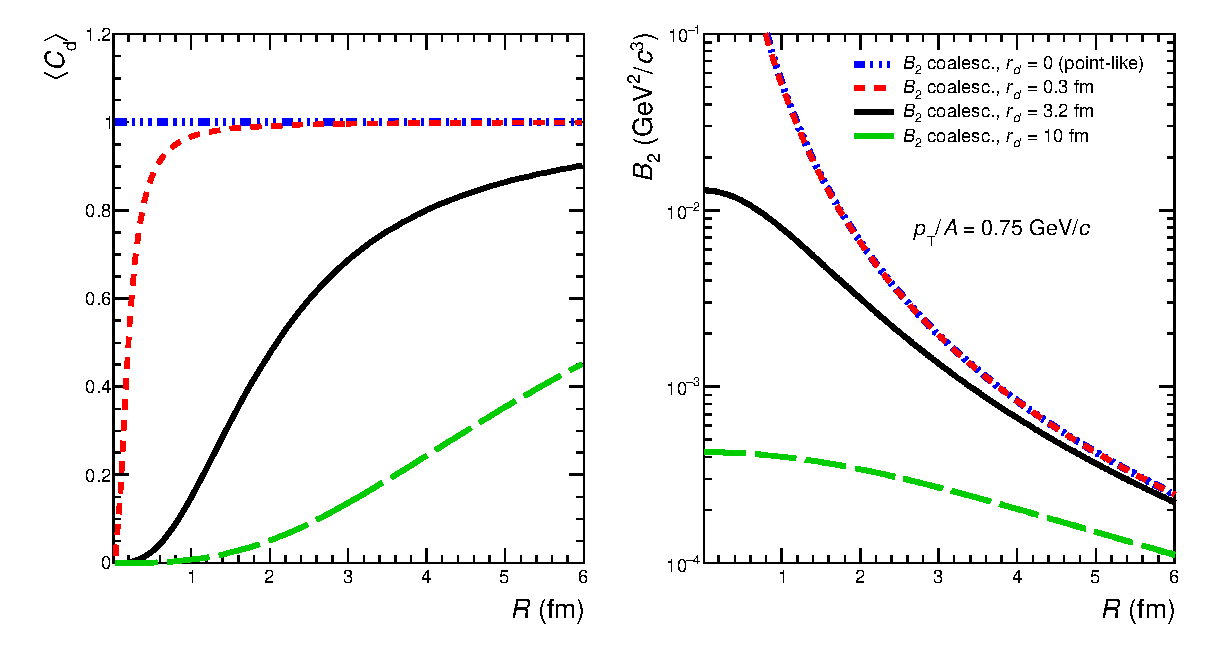
\includegraphics[width=1.0\textwidth]{theory_coalescence_Cd_B2.eps}
\caption{{The quantum mechanical correction factor $\langle C_{d} \rangle$ (left panel, see Eq. \ref{eq:Cdapprox}) and the coalescence parameter \btwo~for deuteron (right panel, see Eq. \ref{eq:B2approx}) as a function of the radius of the source, $R$, calculated assuming a size parameter for the deuteron $\dradius = 0, 0.3, 3.2$ and $10$ fm.}}
\label{fig:radiusDependence}
\end{center}
\end{figure}

Following the approach and discussion presented in~\cite{Blum:2017qnn}, Eq.~\ref{eq:Cd} may be generalised as 

\begin{equation}
\langle C_{A} \rangle = \prod_{i=1,2,3} \left(1 + \frac{r^2}{4R_{i}^2} \right)^{-\frac{1}{2}(A-1)}
\label{eq:CA_general}
\end{equation}
%
for mass number $A$ and the radii $R_{i}$ that describe the volume of the emitting source.
Similarly, the coalescence parameter \bA~for a nucleus with mass number $A$ and spin $J_{A}$ is generalised in \cite{Scheibl:1998tk} as
\begin{equation}
\bA = \frac{2J_{A} +1}{2^{A}}\frac{1}{\sqrt{A}}  \langle C_{A} \rangle \left( \frac{(2\pi)^{3/2}} {m_{T}\prod_{i=1,2,3} R_{i}} \right)^{A-1}.
\label{eq:BA_general}
\end{equation}
In particular, for the case of \hethree~with $A=3$ and $J=1/2$, Eq. \ref{eq:BA_general} becomes the Eq. 9 presented in \cite{Blum:2017qnn}:
\begin{equation}
\bthree = \frac{(2\pi)^{3}}{4\sqrt{3}} \langle C_{3} \rangle (m_{T}\prod_{i=1,2,3} R_{i})^{-2}
\label{eq:B3}
\end{equation}
 
\noindent where

 \begin{equation}
\langle C_{3} \rangle \approx \prod_{i=1,2,3} \left(1 + \frac{r_{3}^2}{4R_{i}^2} \right)^{-1}.
\label{eq:C3}
\end{equation}
 
In summary, under the assumption $R_1\approx R_2 \approx R_3 \approx R$ as in \cite{Blum:2017qnn} (see details in next section) and by combining Eq.~\ref{eq:BA_general} and Eq.~\ref{eq:CA_general}, we obtain the following general expression for the coalescence parameter:

\begin{equation}
	\boxed {  B_{A} = {J_{A} + 1 \over 2^{A}} {1 \over \sqrt{A}} {1 \over m_{T}^{A-1}} \Bigl({2\pi \over R^2 + ({r_A \over 2})^2 }\Bigr)^{3/2(A-1)} } \;\; .
\end{equation}

\noindent This formula can be used to compare the predicted $B_{A}$ with experimental data directly.
 

\subsection{Source volume}
\label{SecSourceVolume}
We identify the source volume as the effective sub-volume of the whole system that is governed by the homogeneity length of the interacting nucleons, as in \cite{Scheibl:1998tk}. In addition, the same authors claim that this volume is experimentally accessible with Hanbury-Brown-Twiss (HBT) interferometry. 
The experimental results are typically obtained following the Bertsch-Pratt (BP) parameterisation ($R_{out}, R_{side}, R_{long}$), while the coalescence model described in Section \ref{sec:coalescence} expresses the volume in terms of the Yano-Koonin-Podgoretskii (YKP) parameterisation. As discussed in Appendix \ref{appendix:YKP}, we identify $\rperp = R_{side}$ and $\rpar = R_{long}$. We then take $R = (\rperp^{2}\rpar)^{1/3} \approx (R_{side}^{2}R_{long})^{1/3}$.

Experimentally, the size of the effective volume can be controlled by selecting different collision geometries, i.e. different centrality classes \cite{Abelev:2013qoq}. In heavy-ion collisions the HBT radii are known to scale with the cubic root of the average charged particle multiplicity density \avdNdeta$^{1/3}$ \cite{Adam:2015vna}, and to depend on the pair average transverse momentum $\langle k_{\mathrm{T}}\rangle$ \cite{Aamodt:2011mr}. In the following, we make the simplifying assumption that the scaling with \avdNdeta$^{1/3}$ holds across collision systems, which is approximately fulfilled in data \cite{Adam:2015pya}. In contrast to \cite{Blum:2017qnn}, we therefore do not explicitly use the measured HBT radii in our study, but we derive the radii from the measured \avdNdeta~according to the following relation:

\begin{equation}
R = a \avdNdeta^{1/3} + b
\label{eq:radiusParameterisation}
\end{equation}

The coefficients, $a = 0.339$ and $b = 0.128$ (in units of fm), have been determined by fitting linearly the ALICE data, and the parameterisation is reported in Fig. \ref{fig:radiiparam}. 
The values we obtain by interpolating the geometric mean of the measured radii are consistent with the radii from kaon femtoscopy for $m_{\mathrm{T}} \approx 1$ \GeVc~in low-multiplicity pp collisions \cite{Abelev:2012sq} and the radii from pion femtoscopy in high-multiplicity \PbPb~collisions at the highest available $k_{\mathrm{T}} \approx 0.9$ \GeVc~\cite{Adam:2015vna}. 
The highest $k_{\mathrm{T}}$ bin was chosen as it is closest in $m_{\mathrm{T}}$ to the lowest transverse momentum per nucleon (\pt/$A \approx 0.8$ \GeVc) accessible by ALICE for the measurement of nuclei production. 
Ideally, one would use the proton femtoscopic radii for such a study, but given that these measurements are not  available in all collision systems and centralities, we assume that $m_{\mathrm{T}}$-scaling holds for HBT radii \cite{Adam:2015vja}.

\begin{figure}[htbp]
\begin{center}
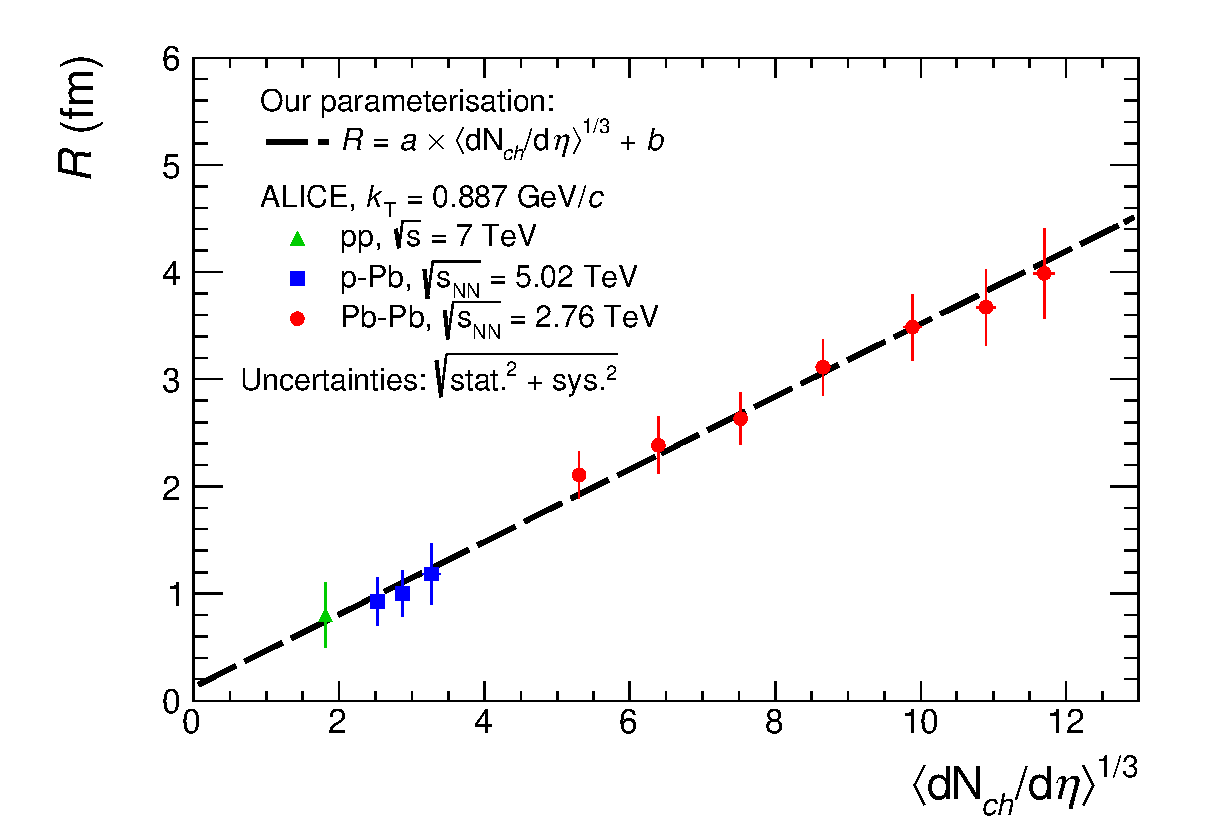
\includegraphics[width=0.7\textwidth]{HbtRadiusParam.eps}
\caption{Parameterisation of the dependence of the source radius on multiplicity assumed in this paper, compared to HBT data from \cite{Adam:2015vna, Adam:2015pya, Abelev:2012sq}. The radius $R$ and the parameters $a$ and $b$ are in units of fm.}
\label{fig:radiiparam}
\end{center}
\end{figure}

\section{Statistical-thermal approach and blast-wave}\label{sec:thermal}

In the statistical-thermal approach, the yields (d$N$/d$y$) of light anti- and hyper-nuclei are very sensitive to the chemical freeze-out temperature $T_{chem}$ due to their large mass $m$ and approximately scale as d$N$/d$y \propto \exp(-m/T_{chem})$. As a matter of fact, the chemical freeze-out temperature defines the only scale in this model, since at the LHC the chemical potentials which ensure the conservation of baryon number ($\mu_{B}$), strangeness ($\mu_{S}$), and electric charge ($\mu_{Q}$) are negligible.
In contrast to the coalescence approach, the current implementations~\cite{Petran:2013dva,Wheaton:2004qb,Andronic:2005yp} of the statistical-thermal model provide only \pt-integrated yields and not the \pt-differential hadron spectra. 
In order to fill this gap, and for the purposes of this exercise, \pt~spectra have been modelled using a blast-wave~\cite{Schnedermann:1993ws} parameterization. When extracting the predicted spectrum for a given particle species (proton, $\Lambda$, deuteron, \hethree), the parameters of the blast-wave (average radial flow velocity $\langle\beta_{T}\rangle$, kinetic freeze-out temperature $T_{kin}$, and velocity profile $n$) are fixed to the values obtained from the simultaneous fit to the pion, kaon and proton spectra measured in Pb--Pb collisions as a function of centrality by ALICE~\cite{Abelev:2013vea}. 
The normalisation is fixed using the \pt-integrated deuteron-to-pion ratio and \hethree-to-pion ratio predicted by the GSI-Heidelberg model with $T_{chem} = 156$ MeV, multiplied by the pion yield measured by ALICE~\cite{Abelev:2013vea}. 
This choice, as opposed to using ratio to proton, is motivated by the fact that the measured proton yield is seen to be slightly underestimated by the thermal model predictions at the LHC~\cite{Abelev:2012wca}.
In the case of hyper-triton, a slightly different procedure is chosen, namely the normalisation for \hthreelambda~is extracted from the statistical-thermal model prediction of the strangeness population factor $S_{3}$ multiplied by the measured $\Lambda/p$ ratio~\cite{Abelev:2013vea,Abelev:2013xaa} and the measured \hethree~yield~\cite{ALICE:deuteronppPbPb2015}. Based on the spectra obtained in this way, we calculate the corresponding coalescence parameters for a given \pt/$A$ and compare it with coalescence expectations. Because we use experimental data to constrain the blast-wave prediction as well as the normalisation, and because such data are provided for given centrality classes, we use the corresponding \avdNdeta~in each class to estimate the system radius based on the parameterisation discussed in Sec.~\ref{SecSourceVolume}. 
In contrast to the coalescence approach, which explicitly depends on the size of the produced object with respect to the system size, the object size does not enter in the formulation of the blast-wave model. Being a simplified hydrodynamic model, the latter treats the system as a continuum and is not particle based. The thermal model on the other hand, implements eigenvolume corrections by fixing the object radius as an external parameter ($r=0.3$~fm in the case of baryons for the GSI-Heidelberg model used here). We refer to the literature for the extensive discussions on the validity of the eigenvolume correction for light anti- and hyper-nuclei~\cite{Vovchenko:2016mwg} and the relation with the possible production of these objects as compact quark bags~\cite{Andronic:2017}.


\section{Comparison with experimental data}\label{sec:comparison}

\subsection{Constraining the source volume with data}\label{sec:radiiParamet}

Data on anti- and hyper-nuclei production at LHC energies and different collision systems have been released by the ALICE Collaboration in recent years \cite{ALICE:nucleipp2017,ALICE:deuteronppPbPb2015,Acharya:2017dmc, Adam:2015yta}. 
In Fig. \ref{fig:CompareB2B3forDifferentParamWithData} we compare the coalescence parameter for deuteron (\btwo) from the coalescence model (see Eqs.~\ref{eq:B2cd} and \ref{eq:B2approx}, with $r_{d} = 3.2$ fm) to the ALICE data for Pb-Pb collisions at $\sqrt{s_{\mathrm{NN}}} = 2.76$ TeV and pp collisions at $\sqrt{s} = 7$ TeV. For pp collisions, data in  \cite{ALICE:nucleipp2017} are given for inelastic (INEL) collisions. In order to facilitate the comparison with future multiplicity-dependent data given in the INEL$>0$ class, we have rescaled the \btwo~and \bthree~by the ratio of the charged particle multiplicity density in these two event classes \cite{Adam:2015gka}.
First, the parameterisation of the system radius fitted to the HBT data as described in Sec.~\ref{SecSourceVolume} (labeled in the following as "parameterisation A") is used to map the \avdNdeta~to the source size (top left panel of Fig. \ref{fig:CompareB2B3forDifferentParamWithData}). 
We notice already at this point that the coalescence volume from parameterisation A radii leads to discrepancies with respect to the curve from the coalescence calculation, and in particular, we notice that the model would require a larger radius for a given value of \btwo~for Pb-Pb collisions.

In a second step the radius is tuned such that the data points for (anti-)deuterons fall onto the coalescence prediction (top right panel of Fig. \ref{fig:CompareB2B3forDifferentParamWithData}). We find that the parameters of Eq.~\ref{eq:radiusParameterisation} turn out to be $a = 0.473$ and $b = 0$. 
With this second parameterisation (labeled as "B" in the following), we investigate the agreement of the model with the measured coalescence parameter for \hethree,  \bthree. As shown in the lower panels of Fig.~\ref{fig:CompareB2B3forDifferentParamWithData}, also in the case of \bthree, a tension between the model and the data is found for parameterisation A, which ameliorates for the parameterisation B, tuned to the (anti-)deuteron data. The strength of this approach is given by the fact that the coalescence volume is constrained with the more differential (anti-)deuteron data assuming that the latter is the same for all anti- and hyper-nuclei. It is also noteworthy that any change of the radii parameterisation would result in a shift along the x axis of both \btwo~and \bthree~data points in the same way, while the theoretical coalescence curve would not be affected. 
 
\begin{figure}[htbp]
	\begin{center}
		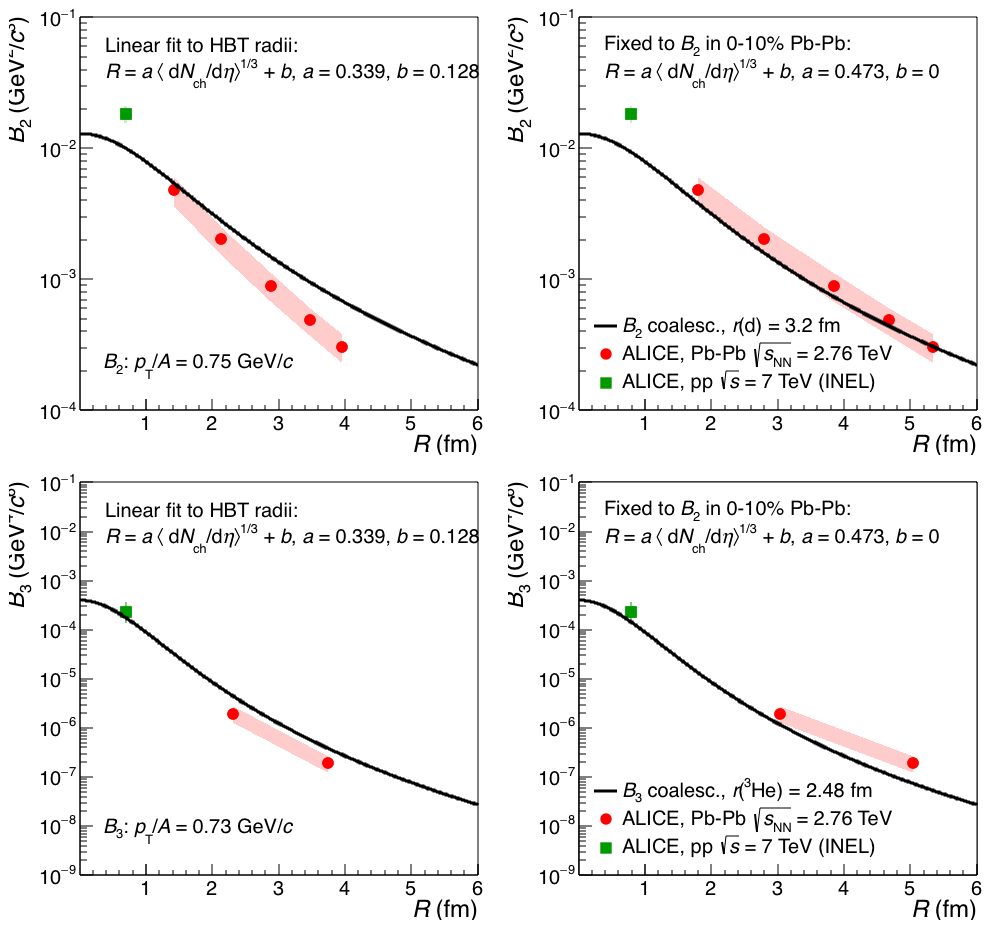
\includegraphics[width=\textwidth]{radiiParamCompareData.png}
		\caption{Comparison of the ALICE data from~\cite{ALICE:nucleipp2017, ALICE:deuteronppPbPb2015} with the coalescence prediction for two different mappings of the \avdNdeta~to the system size $R$: (left panels) the parameterisation A, fitted to the HBT radii, (right panels) the parameterisation B, tuned to the \btwo~values in central Pb-Pb collisions. The radius $R$ and the parameters $a$ and $b$ are in units of fm.}
		\label{fig:CompareB2B3forDifferentParamWithData}
	\end{center}
\end{figure}

\newpage
 \subsection{Thermal and coalescence model for $\mathbf{A = 2, 3}$ anti- and hyper-nuclei}

In Fig.~\ref{fig:CompareThermalAndCoalescence}, the available data for (anti-)deuterons, (anti-)\hethree\ and \hthreelambda~\cite{Adam:2015yta} are compared to both coalescence and thermal model predictions. For the coalescence predictions, the radius parameterisation B is used, as discussed in Sec.~\ref{sec:radiiParamet}. The combined thermal model and blast-wave predictions are calculated as described in Sec.~\ref{sec:thermal}. 

\begin{figure}[ht]
	\begin{center}
		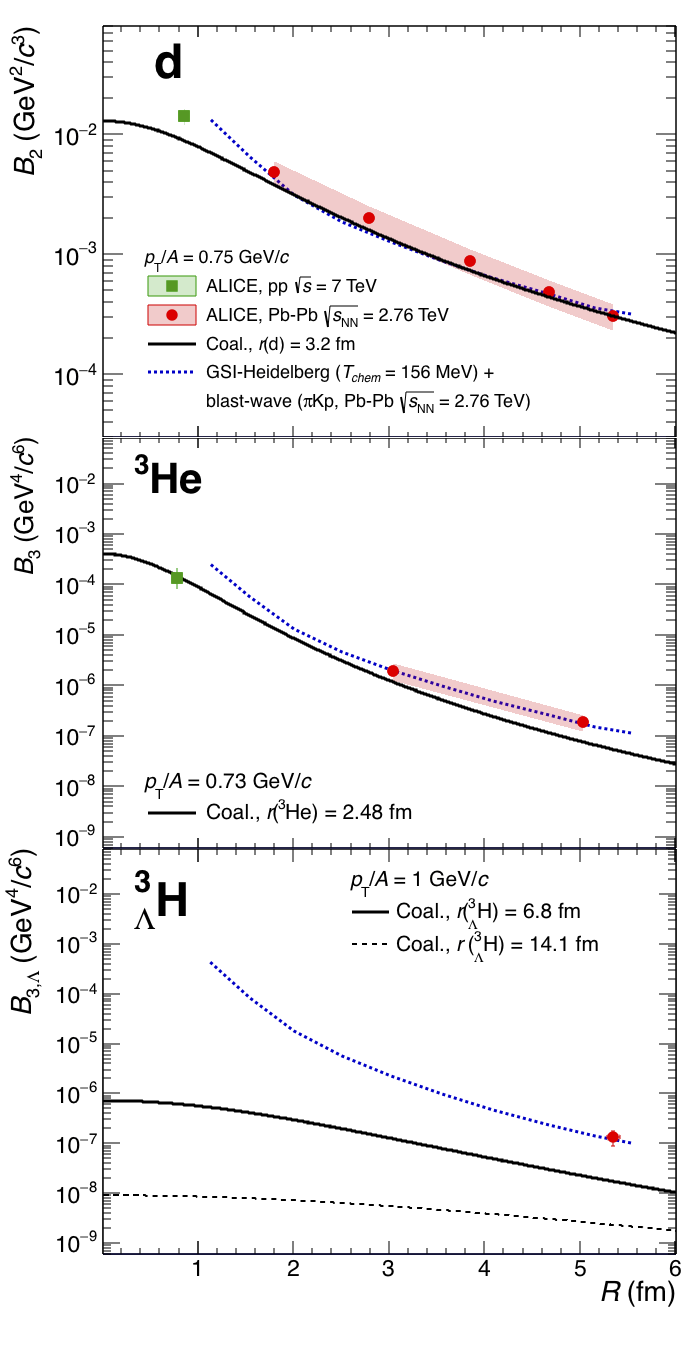
\includegraphics[width=0.8\textwidth]{compareThermalAndCoalescence.png}
		\caption{Comparison of the coalescence parameters measured by ALICE (solid markers) for deuterons (upper left panel), \hethree\ (lower left panel) and \hthreelambda\ (lower right panel) in pp \cite{ALICE:nucleipp2017} and Pb--Pb~\cite{ALICE:deuteronppPbPb2015, Adam:2015yta} collisions with the thermal+BW model expectations (dotted line) and the coalescence predictions (solid lines). Parameterisation B has been used to map the charged particle multiplicity density into the radius $R$ of the source (see text for details). The dashed line in the lower right panel corresponds to the coalescence prediction for the \hthreelambda\ with a larger radius.}
		\label{fig:CompareThermalAndCoalescence}
	\end{center}
\end{figure}

As a first observation, one sees that for deuterons both approaches lead to similar predictions and give a reasonable description of the experimental data for $R \gtrsim 1.6$ fm. 
For \hethree~the two models exhibit a qualitatively similar trend as a function of $R$, but they differ by a factor of about 2. The the limited amount of data that is currently available is consistent with both models within 2$\sigma$ to 3$\sigma$, where $\sigma$ is the total uncertainty on the data. 
Both approaches show large differences (a factor 5 to 6 for central Pb--Pb collisions and a factor of about 30 for small radii, $R < 2$ fm) for the \hthreelambda\ caused by the significantly larger size of \hthreelambda\ with respect to \hethree. 
As a matter of fact, the only datapoint available so far in Pb--Pb collisions is in agreement with the thermal+BW model but not with coalescence. The difference between data and the coalescence model is about 6$\sigma$. However, it is to be kept in mind that the considerations expressed here are subject to the validity of our assumptions, \textit{in primis} the usage of a gaussian form for the wave-function.
Some authors argue that the difference of data to the coalescence model might be explained by a later formation through the coalescence of $\Lambda$s and deuterons~\cite{Zhang:2018euf}. 
In addition, the presence of an excited state with $J=3/2$ of the hyper-triton would significantly enhance the phase space for its production. This is not considered here as there is no evidence for the existence of such an excited state~\cite{Mart:1996ay}. According to our understanding, in both the coalescence and the thermal model calculations the presence of excited states enters via a spin degeneracy factor $(2J_{A}+1)$ and thus the predictions would increase by the same factor.

Most importantly, Fig.~\ref{fig:CompareThermalAndCoalescence} shows that the difference between the two approaches increases with decreasing source volume, thus underlining the need for additional and more precise data as a function of multiplicity or centrality in order to distinguish between the two production scenarios. 
In the case of \hthreelambda~we have considered also a prediction from coalescence for a wider wave-function (dashed line in bottom right panel of Fig. \ref{fig:CompareThermalAndCoalescence}), which results in even lower production probabilities. This behaviour highlights the unique potential to constrain the wave-function of the particle under study at the moment of its production via precise measurements of the coalescence parameter as a function of the source volume. The curves presented here also explicitly allow for an estimate of the expected hyper-triton production in pp collisions. As it can be seen, the latter is expected to be suppressed by about two orders of magnitude with respect to the production of \hethree, thus making this measurement a prime candidate for future experimental studies.
 
 
\section{Summary, conclusions, and outlook}

While it is often argued that the coalescence and the thermal model approach give very similar predictions for the production of light anti- and hyper-nuclei in heavy-ion collisions, the study presented here shows that large differences can be expected for hyper-nuclei with extended wave-functions. In the following, we summarise our main conclusions:
\begin{enumerate}
	\item For the production of $A=2$ and $A=3$ (anti-)nuclei in heavy-ion collisions, the thermal and coalescence models give similar predictions for a source volume that is constrained by experimental data on (anti-)deuteron production in central Pb--Pb collisions at the LHC.
	\item For the production of hyper-triton, the thermal and coalescence models give very different predictions as a function of source volume. In particular, the yield of hyper-tritons appears to be suppressed by about two orders of magnitude in pp collisions with respect to the production of \hethree. The very limited amount of data currently available favours the thermal model prediction within our assumptions.
	\item Systematic measurements in pp, p--Pb, and Pb--Pb collisions at LHC energies have a unique potential to clarify the production mechanism and the nature of composite QCD objects. 
\end{enumerate}

We would like to remark that our study is deliberately based on many simplified assumptions in order to allow for a completely analytical treatment of the problem. Future studies should be based on more realistic approximations, which requires numerical calculations. Moreover, as the study presented here has been carried out for a specific value of transverse momentum per nucleon, it will be interesting to explore further the \pt~dependence of the observations made here in comparison to future and currently available data.

In a follow-up publication, we plan to extend our study to predictions for the $A=4$ systems introduced in Tab.~\ref{tab:nucleusradii} and to more exotic QCD objects like the X(3872). In fact, if the X(3872) corresponds to a loosely bound $\overline{D}^{*0}$--$D^{0}$ molecule, the rms of its wave-function can be as large as $4.9^{+13.4}_{-1.4}$~fm \cite{Artoisenet:2010uu}, which is very similar to that of the hyper-triton. Thus, its possible production via a coalescence mechanism in pp collisions would be subject to a similar suppression as the hyper-triton. Additional theoretical studies and numerical predictions are encouraged in view of the high-luminosity phase of the LHC (Run 3 $\&$ 4), where $A = 4$ hyper-nuclei and other rare composite objects might become experimentally accessible.


%%%%%%%%%%%%%%%%%%%%%%%%%%%%%%%%%%%%%%%%%
% acknowledgments
%%%%%%%%%%%%%%%%%%%%%%%%%%%%%%%%%%%%%%%%%

\newenvironment{acknowledgement}{\relax}{\relax}
\begin{acknowledgement}
\section*{Acknowledgements}
We thank U. Heinz for the useful discussions and the clarification on the equivalence of the Bertsch-Pratt and Yano-Koonin-Podgoretskii parameterisations of the HBT radii. We further acknowledge discussions with Benjamin Doenigus, in particular about the production of \hthreelambda\ in pp collisions. In addition, we would like to thank Juergen Schukraft, Peter Braun-Munzinger, Roman Lietava, Kfir Blum and the colleagues from the ALICE Collaboration for their valuable input.  

\end{acknowledgement}


%%%%%%%%%%%%%%%%%%%%%%%%%%%%%%
%   APPENDIX                   
%%%%%%%%%%%%%%%%%%%%%%%%%%%%%%
\begin{appendix}
\section{Relation to the Sato-Yazaki coalescence model}\label{appendix:Sato}
The approach of Sato and Yazaki~\cite{Sato:1981ez} is based on a density matrix model and includes explicitly the system size dependence and wave-function dependence of the coalescence process albeit it assumes a sudden approximation when particles cease their interactions (sudden freeze-out) and thus neglects the collective expansion of the medium in contrast to~\cite{Scheibl:1998tk}. It assumes no correlation between different nucleons and no correlation between coordinates in space and momentum. In a heavy ion collisions, such correlations are consequence of hydrodynamical flow. 
The coalescence process to form a nucleus with mass number $A = Z + N$ is formulated in terms of the momentum per nucleon ($p$) as
%
\begin{equation}
\frac{\gamma_{A}}{\sigma_{A,0}} \frac{d^{3}\sigma_{A}}{d^{3}p} =  \left( {4 \over 3} \pi p_{0}^{3}\right)^{A-1}\frac{1}{Z! N!} \left(\frac{\gamma_{p}}{\sigma_{p,0}} \frac{d^{3}\sigma_{p}}{d^{3}p_{p}}\right)^{Z} \left(\frac{\gamma_{n}}{\sigma_{n,0}} \frac{d^{3}\sigma_{n}}{d^{3}p_{n}}\right)^{N} 
\end{equation} 
%
where $p_{0}$ corresponds to the coalescence momentum, $\gamma_{A}$ and $\gamma_{p,n}$ are the Lorentz factors for the nucleus and the nucleons, respectively. The reaction cross sections are denoted as $\sigma_{i,0}$, where $A = p, n, A$.
Assuming that the proton and neutron emission probabilities are equal and that $p_{p} \approx p_{n} \equiv p$, this expression relates to the $B_{A}$ as defined by our Lorentz invariant Eq.(\ref{eq:BA}) as

\begin{equation}
B_{A} = \left({4 \over 3} \pi p_{0}^{3}\right)^{A-1} {M \over m^{A}} {1 \over A^{3}}{\frac{1}{Z! N!}}
\end{equation}

\noindent where the factor ${1 \over A^{3}}$ results from the transformation of $p_{A} \rightarrow A p_{p,n}$ and $M$ corresponds to the nucleus mass and $m$ to the nucleon mass. This expression can be further simplified via the approximation $M \approx A m$ to

\begin{equation}
B_{A} = \left({4 \over 3} \pi p_{0}^{3}\right)^{A-1} {1 \over m^{A-1}} {1 \over A^{2}}{\frac{1}{Z! N!}} \; .
\end{equation}

\noindent For nuclei up to $A = 4$ and the non-relativistic case, Sato and Yazaki derive the following relations for the coalescence momentum $p_{0}$, 
%
\begin{align}
	A& =2&
	{4 \over 3} \pi p_{0}^{3}& ={3 \over 4}2^{3/2}(4\pi)^{3/2} \left(\frac{\nu_{2}\nu}{\nu_{2} + \nu}\right)^{3/2}\\
	A& =3&
	{1 \over 2} \left( {4 \over 3} \pi p_{0}^{3}\right)^{2}& ={1 \over 4} 3^{3/2} (4\pi)^{3} \left(\frac{\nu_{3}\nu}{\nu_{3} + \nu}\right)^{3}\\
	A& =4&  
	{1 \over 4} \left({4 \over 3} \pi p_{0}^{3}\right)^{3}& = {1 \over 16} 4^{3/2} (4\pi)^{9/2} \left(\frac{\nu_{4}\nu}{\nu_{4}+ \nu}\right)^{9/2}
\end{align}

\noindent where the size parameter $\nu$ relates to the rms radius $R_{rms}$ of the emission source as $\nu~=~\sqrt{3 \over 2 R_{rms}}$, and $\nu_{A}$ is the size parameter of the nucleus. 
\\Following the generalisation in~\cite{Nagle:1996vp}, we thus propose the following parameterisation for the coalescence parameter

\begin{eqnarray}
B_{A} &=& {2J_{A} + 1 \over 2^{A}} A^{3/2} (4\pi)^{{3\over2}(A-1)} \Bigl({\nu_{A}\nu \over \nu_{A}+ \nu}\Bigr)^{{3\over2}(A-1)} {1 \over m^{A-1}} {1 \over A^{2}}  \\
\label{eq:SatoGeneralised}
           &=&  {2J_{A} + 1 \over 2^{A}} {1 \over m^{A-1}} {1 \over \sqrt{A}} (4\pi)^{{3\over2}(A-1)} \Bigl({\nu_{A}\nu \over \nu_{A}+ \nu}\Bigr)^{{3\over2}(A-1)} \;,
\end{eqnarray}

\noindent indicating with $J_{A}$ the spin of the nucleus.
Once again, the $\nu_{A}$ parameter corresponds to the size parameter of the nucleus wave-function, which is assumed to be gaussian (solution to the isotropic spherical harmonic oscillator potential) of the form~\cite{Sato:1981ez,Bergstrom:1979gpv}:

\begin{equation}\label{eq:SatoWave}
 \phi_{A} = C \exp\Bigl(-{1\over2} \nu_{A} \sum_{i=1}^{A}(\vec{x}_{i} - \vec{X})^2 \Bigr)
\end{equation}

\noindent with an appropriate normalisation factor $C$ and the coordinate vector $\vec{X}$ of the centre-of-mass system. 
 
We have also verified that our generalisation of Sato-Yazaki provided by Eq. \ref{eq:SatoGeneralised} and the expression derived from Heinz in Eq. \ref{eq:CA_general} become consistent in the limit $R_{rms} \approx R \rightarrow 0$ (point-like source) and $p_{\mathrm{T}} \rightarrow 0$ (static source), provided that one identifies $\nu_{A} = {2 / r_{A}^{2}}$. Incidentally, the same relation between $\nu_{A}$ and $r_{A}$ can be derived by a straightforward comparison of the nucleus wave-functions employed by the same authors \cite{Scheibl:1998tk,Sato:1981ez}. 

The parameter $\nu_{A}$ is typically chosen such that the measured rms charge radius \rmsradius~is reproduced. The relation between \rmsradius~and $\nu_{A}$ is obtained by a transformation to the Jacobi variables and performing the integration (see Appendix \ref{appendix:integration}). In particular, one obtains for $A < 5$:

\begin{align}
	A& = 2 \qquad \qquad \nu_{2} = {3 \over {4\rmsd^2}}  \\
	A& = 3 \qquad \qquad \nu_{3} = {1 \over {\rmsthree^2}} \\
	A& = 4 \qquad \qquad \nu_{4} =  {9 \over {8\rmsfour^2}} \;\; .
\end{align}

%%%%%%%%%%%%%%%%%%%%%%%%%%%%%%%%%%%%%%%%%
% A = 4 Appendix
%%%%%%%%%%%%%%%%%%%%%%%%%%%%%%%%%%%%%%%%%
\newpage
\section{RMS of a gaussian wave-function for A=4 }\label{appendix:integration}

In this appendix, we show the calculation of the RMS of a gaussian wave-function with the example of A=4. We start from the wave-function

\begin{equation}\label{eq:SatoWave}
 \phi_{A=4} = C_{4} \exp\Bigl(-{1\over2} \nu_{4} \sum_{i=1}^{4}(\vec{x}_{i} - \vec{X})^2 \Bigr) \; .
\end{equation}

\noindent Then we introduce the Jacobi variables which are given by 
\begin{align}
	\vec{X}    &= {1 \over 4} (\vec{x_1} + \vec{x_2} + \vec{x_3} + \vec{x_4}) \\
	\vec{r_1} &= \vec{x_2} - \vec{x_1}\\
	\vec{r_2} &= \vec{x_3} - {1 \over 2}(\vec{x_1} + \vec{x_2})\\
	\vec{r_3} &= \vec{x_4} - {1 \over 3}(\vec{x_1} + \vec{x_2} + \vec{x_3}) \; .
\end{align}

\noindent In this parameterisation we can express the squared distance of each nucleon with respect to the centre-of-mass as

\begin{equation}
 \sum_{i=1}^{4} \bigl(\vec{x_i} - \vec{X} \bigr)^2 = {1\over 4} \bigl(2\vec{r_1} + {8\over 3}\vec{r_2} + 3\vec{r_3}\bigr)  \; .
\end{equation}

\noindent For the following integral calculations we determine the Jacobian as

\begin{align}
	\mathrm{d}R\mathrm{d}r_{1}\mathrm{d}r_{2}\mathrm{d}r_{3} &= \vert\det {\partial(R,r_{1},r_{2},r_{3}) \over \partial(x_{1},x_{2},x_{3},x_{4})}\vert \; \mathrm{d}x_{1}\mathrm{d}x_{2}\mathrm{d}x_{3}\mathrm{d}x_{4} \\
		&= \begin{vmatrix} {\partial R \over \partial x_{1}} & {\partial r_{1} \over \partial x_{1}} & {\partial r_{2} \over \partial x_{1}}& {\partial r_{3} \over \partial x_{1}} \\ 
		{\partial R \over \partial x_{2}} & {\partial r_{1} \over \partial x_{2}} & {\partial r_{2} \over \partial x_{2}}& {\partial r_{3} \over \partial x_{2}} \\ 
		{\partial R \over \partial x_{3}} & {\partial r_{1} \over \partial x_{3}} & {\partial r_{2} \over \partial x_{3}}& {\partial r_{3} \over \partial x_{3}} \\ 
		{\partial R \over \partial x_{4}} & {\partial r_{1} \over \partial x_{4}} & {\partial r_{2} \over \partial x_{4}}& {\partial r_{3} \over \partial x_{4}} \end{vmatrix} 
		\mathrm{d}x_{1}\mathrm{d}x_{2}\mathrm{d}x_{3}\mathrm{d}x_{4} \\
		&=  \begin{vmatrix} {1\over 4} & -1 & -{1\over 2} & -{1\over 3}  \\
			{1\over 4} & 1 & -{1\over 2} & -{1\over 3}  \\
			{1\over 4} & 0 & 1 & -{1\over 3}  \\
			{1\over 4} & 0 & 0 & 1
			 \end{vmatrix} \mathrm{d}x_{1}\mathrm{d}x_{2}\mathrm{d}x_{3}\mathrm{d}x_{4} \\
		&= 1 \cdot \mathrm{d}x_{1}\mathrm{d}x_{2}\mathrm{d}x_{3}\mathrm{d}x_{4} \; .
\end{align}

\noindent From the requirement $\int|\phi|^2\mathrm{d}\vec{r}_{1}\mathrm{d}\vec{r}_{2}\mathrm{d}\vec{r}_{3} = 1$, we thus obtain for the normalisation constant $C_4$: 

\begin{align}
	{1\over C_{4}^{2}} &= \int \exp^{2}\Bigl(-{1\over 2} \nu_{4} ({1\over 2}r_{1}^{2} + {2\over 3} r_{2}^{2} + {3\over 4}r_{3}^{2}) \Bigr) \mathrm{d}\vec{r}_{1}\mathrm{d}\vec{r}_{2}\mathrm{d}\vec{r}_{3}
\end{align}

\noindent where the integration in spherical coordinates is performed with $\mathrm{d}\vec{r}_{1} = 4\pi r_{1}^{2}\mathrm{d}r_{1},  \mathrm{d}\vec{r}_{2} = \ldots$ which gives

\begin{align}
	{1\over C_{4}^{2}} &= (4\pi)^{3} \underbrace{\int_{0}^{\infty} r_{1}^{2}\exp\Bigl(-{1\over 2} \nu_{4}  r_{1}^{2}  \Bigr)  \mathrm{d}r_{1}}_{{\sqrt{\pi} \over 4} {1 \over ({1\over 2} \nu_{4})^{3/2}}  }
							\underbrace{\int_{0}^{\infty} r_{2}^{2}\exp\Bigl(-{2\over 3} \nu_{4}  r_{2}^{2}  \Bigr)  \mathrm{d}r_{2}}_{{\sqrt{\pi} \over 4} {1 \over ({2\over 3} \nu_{4})^{3/2}}  }
							\underbrace{\int_{0}^{\infty} r_{3}^{2}\exp\Bigl(-{3\over 4} \nu_{4}  r_{3}^{2}  \Bigr)  \mathrm{d}r_{3}}_{{\sqrt{\pi} \over 4} {1 \over ({3\over 4} \nu_{4})^{3/2}}  } \\
		&= \bigl({\pi \over \nu_{A}}\bigr)^{9/2} 4^{3/2} \\
	\Rightarrow C_{4} &= \Bigl({\nu_{A}^{3} \over 4 \pi^{3}}\Bigr)^{3/4} \;.
\end{align}

\noindent For the rms, we obtain accordingly:


\begin{align}
	\lambda_{4}^{2} &= {1 \over 4} \langle \phi \vert   \sum_{i=1}^{4}(\vec{x}_{i} - \vec{X})^2 \vert \phi \rangle \\
	&= \int {1\over 4}  \sum_{i=1}^{4}(\vec{x}_{i} - \vec{X})^2 |\phi|^2 \mathrm{d}\vec{x}_{1}\mathrm{d}\vec{x}_{2}\mathrm{d}\vec{x}_{3}\mathrm{d}\vec{x}_{4} \\
	 &= {C_4^2 \over 4}  \int \bigl({1\over 2}r_{1}^{2} + {2\over 3} r_{2}^{2} + {3\over 4}r_{3}^{2} \bigr) \exp^{2}\Bigl(-{1\over 2} \nu_{4} ({1\over 2}r_{1}^{2} + {2\over 3} r_{2}^{2} + {3\over 4}r_{3}^{2}) \Bigr) \mathrm{d}\vec{r}_{1}\mathrm{d}\vec{r}_{2}\mathrm{d}\vec{r}_{3} \\
	&= {C_4^2 \over 4} \Bigl(\underbrace{{1\over 2} \int r_{1}^2 \exp\bigl(-{1\over2} \nu_A r_{1}^{2}\bigr) \exp\bigl(-{2\over3} \nu_A r_{2}^{2}\bigr) \exp\bigl(-{3\over4} \nu_A r_{3}^{2}\bigr) \mathrm{d}\vec{r}_{1}\mathrm{d}\vec{r}_{2}\mathrm{d}\vec{r}_{3}}_{\mathrm{I}} \\
	&\;\;+ \underbrace{{2\over 3} \int r_{2}^2 \exp\bigl(-{1\over2} \nu_A r_{1}^{2}\bigr) \exp\bigl(-{2\over3} \nu_A r_{2}^{2}\bigr) \exp\bigl(-{3\over4} \nu_A r_{3}^{2}\bigr) \mathrm{d}\vec{r}_{1}\mathrm{d}\vec{r}_{2}\mathrm{d}\vec{r}_{3}}_{\mathrm{II}} \\
	&\;\;+ \underbrace{{3\over 4} \int r_{3}^2 \exp\bigl(-{1\over2} \nu_A r_{1}^{2}\bigr) \exp\bigl(-{2\over3} \nu_A r_{2}^{2}\bigr) \exp\bigl(-{3\over4} \nu_A r_{3}^{2}\bigr) \mathrm{d}\vec{r}_{1}\mathrm{d}\vec{r}_{2}\mathrm{d}\vec{r}_{3}}_{\mathrm{III}}
				 \Bigr)
\end{align}

\noindent The first summand I can be calculated with $\mathrm{d}\vec{r}_{1}\mathrm{d}\vec{r}_{2}\mathrm{d}\vec{r}_{3} = (4\pi)^3 r_1^2 r_2^2 r_3^2 \mathrm{d}r_{1}\mathrm{d}r_{2}\mathrm{d}r_{3}$ as

\begin{align}
 \mathrm{I} &= {1\over 2} (4\pi)^3 \cdot \int_{0}^{\infty} r_{1}^2 \exp\bigl(-{1\over2} \nu_A r_{1}^{2}\bigr)\mathrm{d}r_{1} \cdot \int_{0}^{\infty}\exp\bigl(-{2\over3} \nu_A r_{2}^{2}\bigr) \mathrm{d}r_{2} \cdot \int_{0}^{\infty} \exp\bigl(-{3\over4} \nu_A r_{3}^{2}\bigr) \mathrm{d}r_{3} \\
 	&= {1\over 2} (4\pi)^3 \cdot {3\sqrt{\pi} \over 8} {1 \over ({1\over 2} \nu_{A})^{5/2}} \cdot {\sqrt{\pi} \over 4} {1 \over ({2\over 3} \nu_{A})^{3/2}} \cdot {\sqrt{\pi} \over 4} {1 \over ({3\over 4} \nu_{A})^{3/2}} \;.
\end{align}

\noindent The other two summands II and III are evaluated accordingly and we thus obtain for the rms:

\begin{align}
	\lambda_{4}^{2} &= {C_4^2 \over 4} (\mathrm{I} + \mathrm{II} + \mathrm{III} ) \\
	&= {C_4^2 \over 4} (4\pi)^3 {3\pi^{3/2} \over 8 \cdot 4^2 \cdot \nu_A^{11/2}} \underbrace{\Bigl({{1\over2} \over ({1\over2})^{5/2}({2\over3})^{3/2}({3\over4})^{3/2} } +
	{{2\over3} \over ({1\over2})^{3/2}({2\over3})^{5/2}({3\over4})^{3/2} } + {{3\over4} \over ({1\over2})^{3/2}({2\over3})^{3/2}({3\over4})^{5/2} } \Bigr)}_{= 24} \\
	&= {9 \over 8 \nu_A} \;.
\end{align}

%%%%%%%%%%%%%%%%%%%%%%%%%%%%%%%%%%%%%%%%%
% HBT Appendix
%%%%%%%%%%%%%%%%%%%%%%%%%%%%%%%%%%%%%%%%%
\newpage
\section{HBT radii in Bertsch-Pratt and Yano-Koonin-Podgoretskii parameterisation for comparison with coalescence models}\label{appendix:YKP}

The results of HBT analyses are typically presented in either the Bertsch-Pratt ($R_{out}$, $R_{side}$, $R_{long}$) or the Yano-Koonin-Podgoretskii ($R_{\perp}$, $R_{0}$, $R_{\parallel}$) parameterization. The ALICE HBT results \cite{Aamodt:2011mr, Adam:2015vna} are given in the Bertsch-Pratt convention, whereas the coalescence parameter is derived in \cite{Scheibl:1998tk} by expressing the dependence on the volume in terms of the Yano-Koonin-Podgoretskii (YKP) parameterisation. 
The transformation between the two parameterisations is best presented in~\cite{Wiedemann:1999qn} in the equations (W 3.48) to (W 3.52)\footnote{The equations in~\cite{Wiedemann:1999qn} are denoted as (W...) in order to distinguish them from the equations presented in this paper.}:

\begin{eqnarray}
R_{side}^{2}    &=& R_{\perp}^{2}  \;, \\
R_{diff}^{2} &=& R_{out}^{2} -  R_{side}^{2} = \beta_{\perp}^2 \gamma^2 (R_{0}^2 + v^2R_{\parallel}^2) \;, \\
R_{long}^{2}     &=& (1 - \beta_l^2) R_{\parallel}^2 + \gamma^2 (\beta_l - v)^2 (R_{0}^2 + v^2R_{\parallel}^2) \;, \\
R_{ol}^{2}   &=& \beta_{\perp} (-\beta_l R_{\parallel}^{2} +  \gamma^2 (\beta_l - v)(R_{0}^2 + v^2R_{\parallel}^2)) \,.
\end{eqnarray}
%
We immediately identify that $R_{\perp}^2$ can be identified with $R_{side}^{2}$. Following the reasoning and the nomenclature in~\cite{Wiedemann:1999qn} (W 3.52-3.53), the above equations can be inverted and $R_{\parallel}^{2}$ can be expressed as 
%
\begin{eqnarray}
R_{\parallel}^{2} &=& B  - v \cdot C \;, \\
                          &=& R_{long}^2 - 2{\beta_l \over \beta_\perp}  R_{ol}^2 + {\beta_l^2 \over \beta_\perp^2} R_{diff}^2 
                          - v \cdot \Bigl(-{1 \over \beta_\perp } R_{ol}^2 + {\beta_l \over \beta_\perp^2} R_{diff}^2  \Bigr) \; .
\end{eqnarray}
%
As it turns out all corrections which are subtracted from $R_{long}^{2}$ can be neglected. First, we notice that the cross term $R_{ol}$ vanishes if the measured fireball is longitudinally boost-invariant, which is a valid approximation for the rapidity ranges studied here. The remaining terms are all proportional to $\beta_l$. By definition of the rest frame for a longitudinally-boosted invariant system, $\beta_l = 0$. In summary, we can consider $R_{\perp} = R_{side}$ and $R_{\parallel}=R_{long}$ for the present study.


\end{appendix}

\bibliographystyle{utphys} 	
\bibliography{NucleiB2}

\end{document}

